\documentclass[aspectratio=169]{beamer}
\setbeamertemplate{navigation symbols}{}
\usepackage{color, amsmath, comment, subfigure}
\usepackage{url}

\usepackage{hyperref}
\hypersetup{
    colorlinks=true,
    linkcolor=blue,
    filecolor=magenta,      
    urlcolor=cyan,
}

%%%%%%%%%%%%%%%%%%%%%%%%%%
\title[]{Class slides for Thursday, Sept 24:\\Armed conflict, part 2}
\author[]{Matthew J. Salganik}
\institute[]{}
\date[]{COS 597E/SOC 555 Limits to prediction\\Fall 2020, Princeton University}

\begin{document}
%%%%%%%%%%%%%%%%%%%%%%%%%%%
\frame{\titlepage}
%%%%%%%%%%%%%%%%%%%%%%%%%%%
\begin{frame}
\frametitle{}

\begin{center}
\only<1>{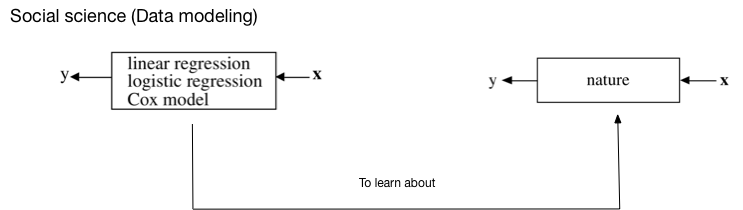
\includegraphics[width=0.9\textwidth]{figures/third_way_1}}%
\only<2>{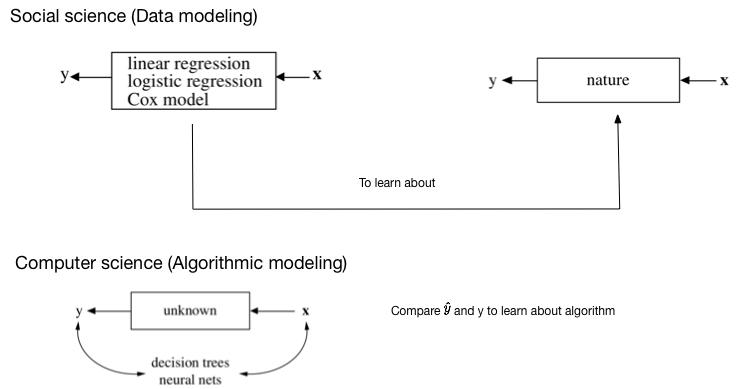
\includegraphics[width=0.9\textwidth]{figures/third_way_2}}%
\only<3>{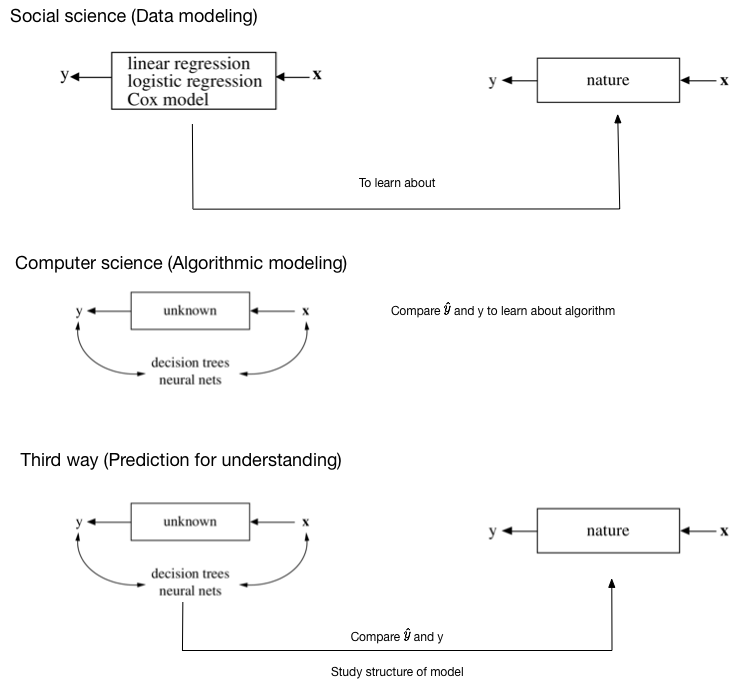
\includegraphics[width=0.6\textwidth]{figures/third_way_3}}%
\end{center}

\end{frame}
%%%%%%%%%%%%%%%%%%%%%%%%%%%
\begin{frame}
\frametitle{}

\begin{center}
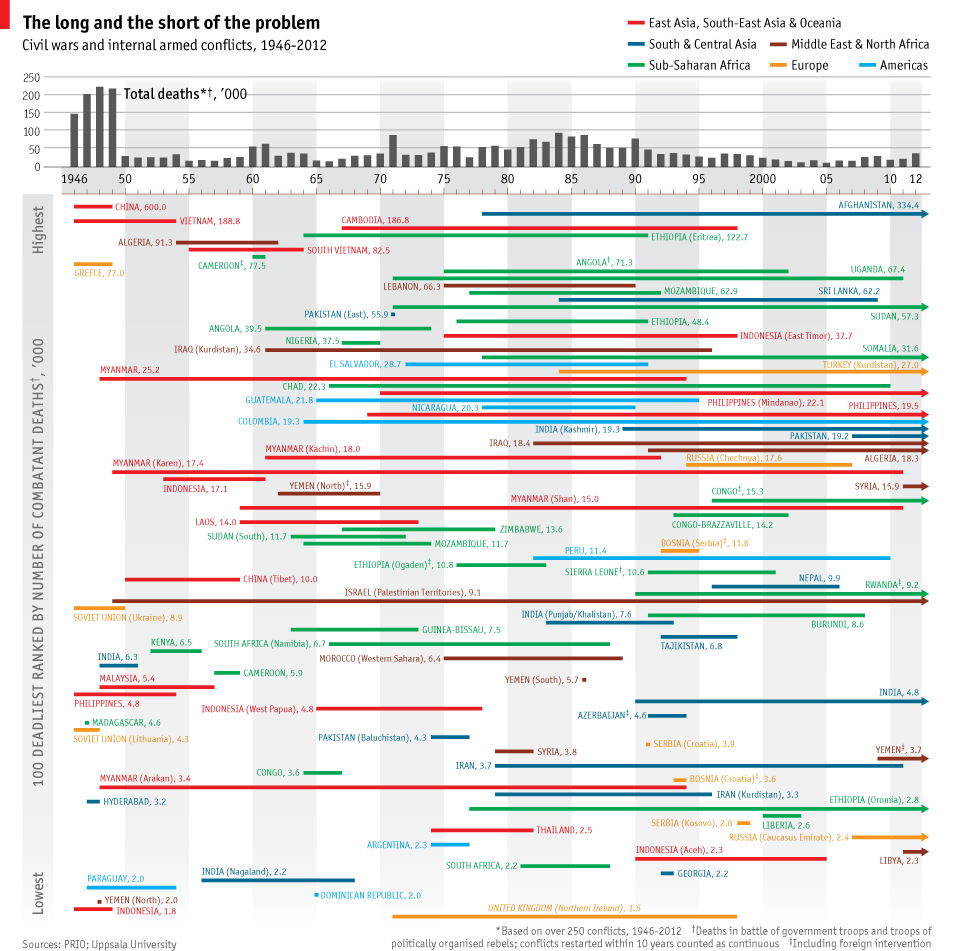
\includegraphics[height=0.9\textheight]{figures/ourworldindata_the-100-deadlist-civil-wars-the-economist}
\end{center}

\vfill
\tiny{\url{https://www.economist.com/content/inner-turmoil}}
% focus on onset
\end{frame}
%%%%%%%%%%%%%%%%%%%%%%%%%%%%
\begin{frame}
\frametitle{}

\begin{center}
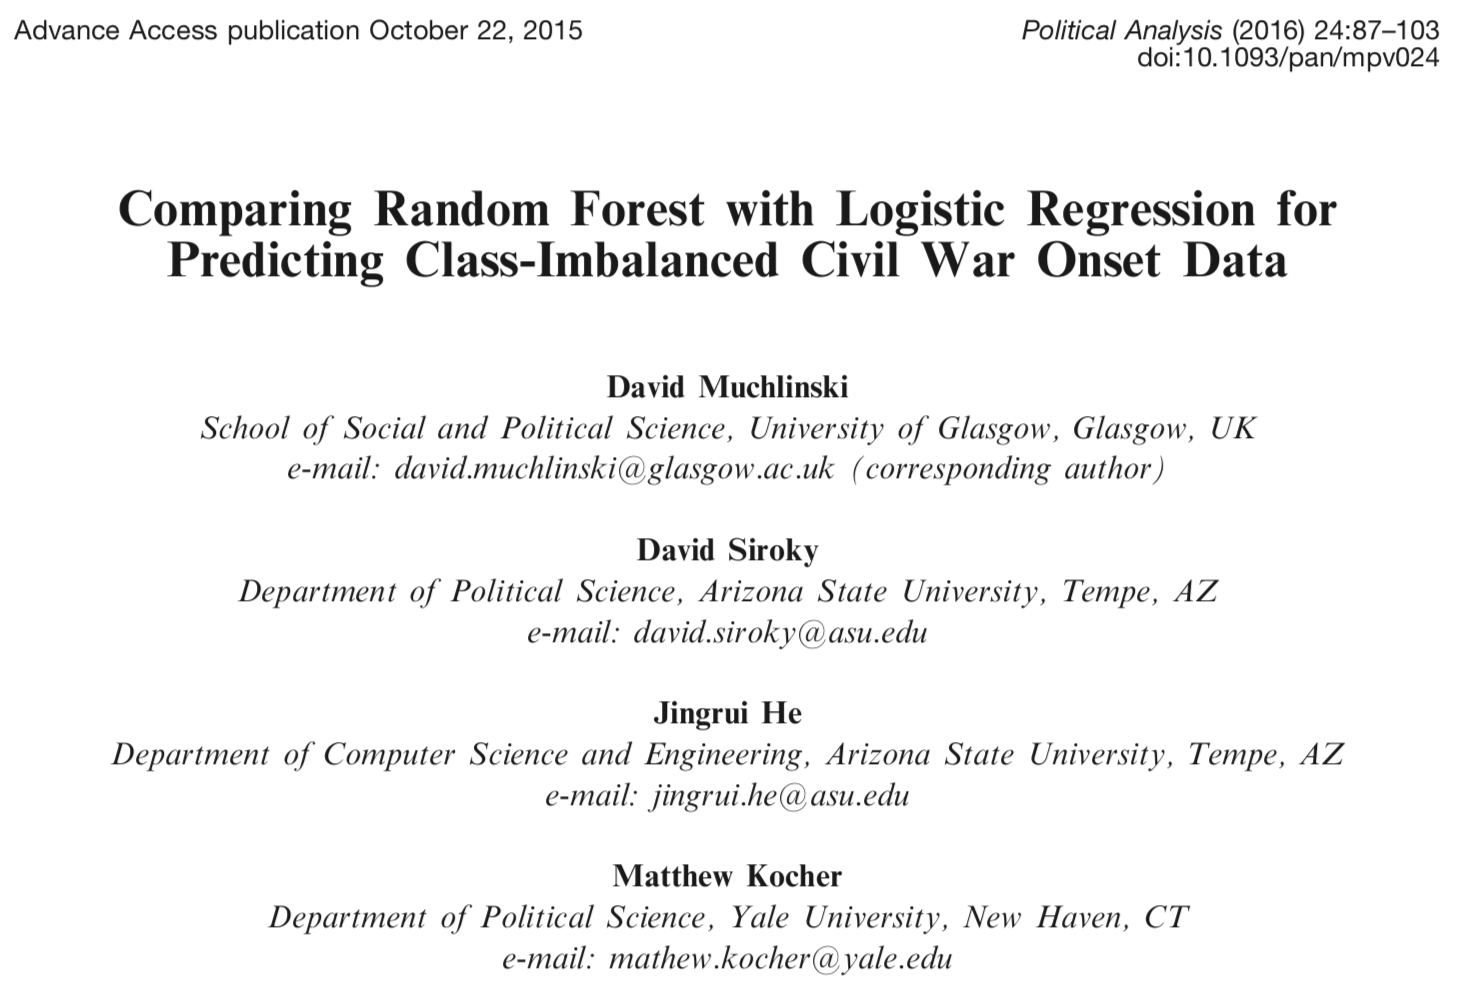
\includegraphics[width=0.9\textwidth]{figures/muchlinksi_comparing_2016_title}
\end{center}

\end{frame}
%%%%%%%%%%%%%%%%%%%%%%%%%%%
\begin{frame}
\frametitle{}

\begin{itemize}
\item Two goals: (1) compare random forest to logistic regression for predicting civil war onset (2) learn from random forest about civil war onset.
\pause
\item Regarding goal (1):
\begin{itemize}
\item This feels like a weird hybrid. If you are going to argue for prediction, why not go all in? (Schelling wind tunnel story)
\pause
\item I find the comparison between random forest and logistics regression misleading because two things are varying: number of predictors and learning algorithm. \pause Better way might be to keep the predictor set fixed.
\pause 
\item A lot of work has already happened in both feature selection and feature engineering (e.g., GDP growth and GDP per capita) before random forest is ever used
\pause
\item They did not model the panel data structure (e.g., no country fixed effects).  Why? If the goal is to help policy makers, then we should allow country fixed effects.
\pause
\item Starts like a paper about onset of civil wars, ends like a paper about random forest
\pause
\item Notice that models did not maximize scoring function (AUC)
\end{itemize}
\end{itemize}

\end{frame}
%%%%%%%%%%%%%%%%%%%%%%%%%%%%
\begin{frame}
\frametitle{}

\begin{center}
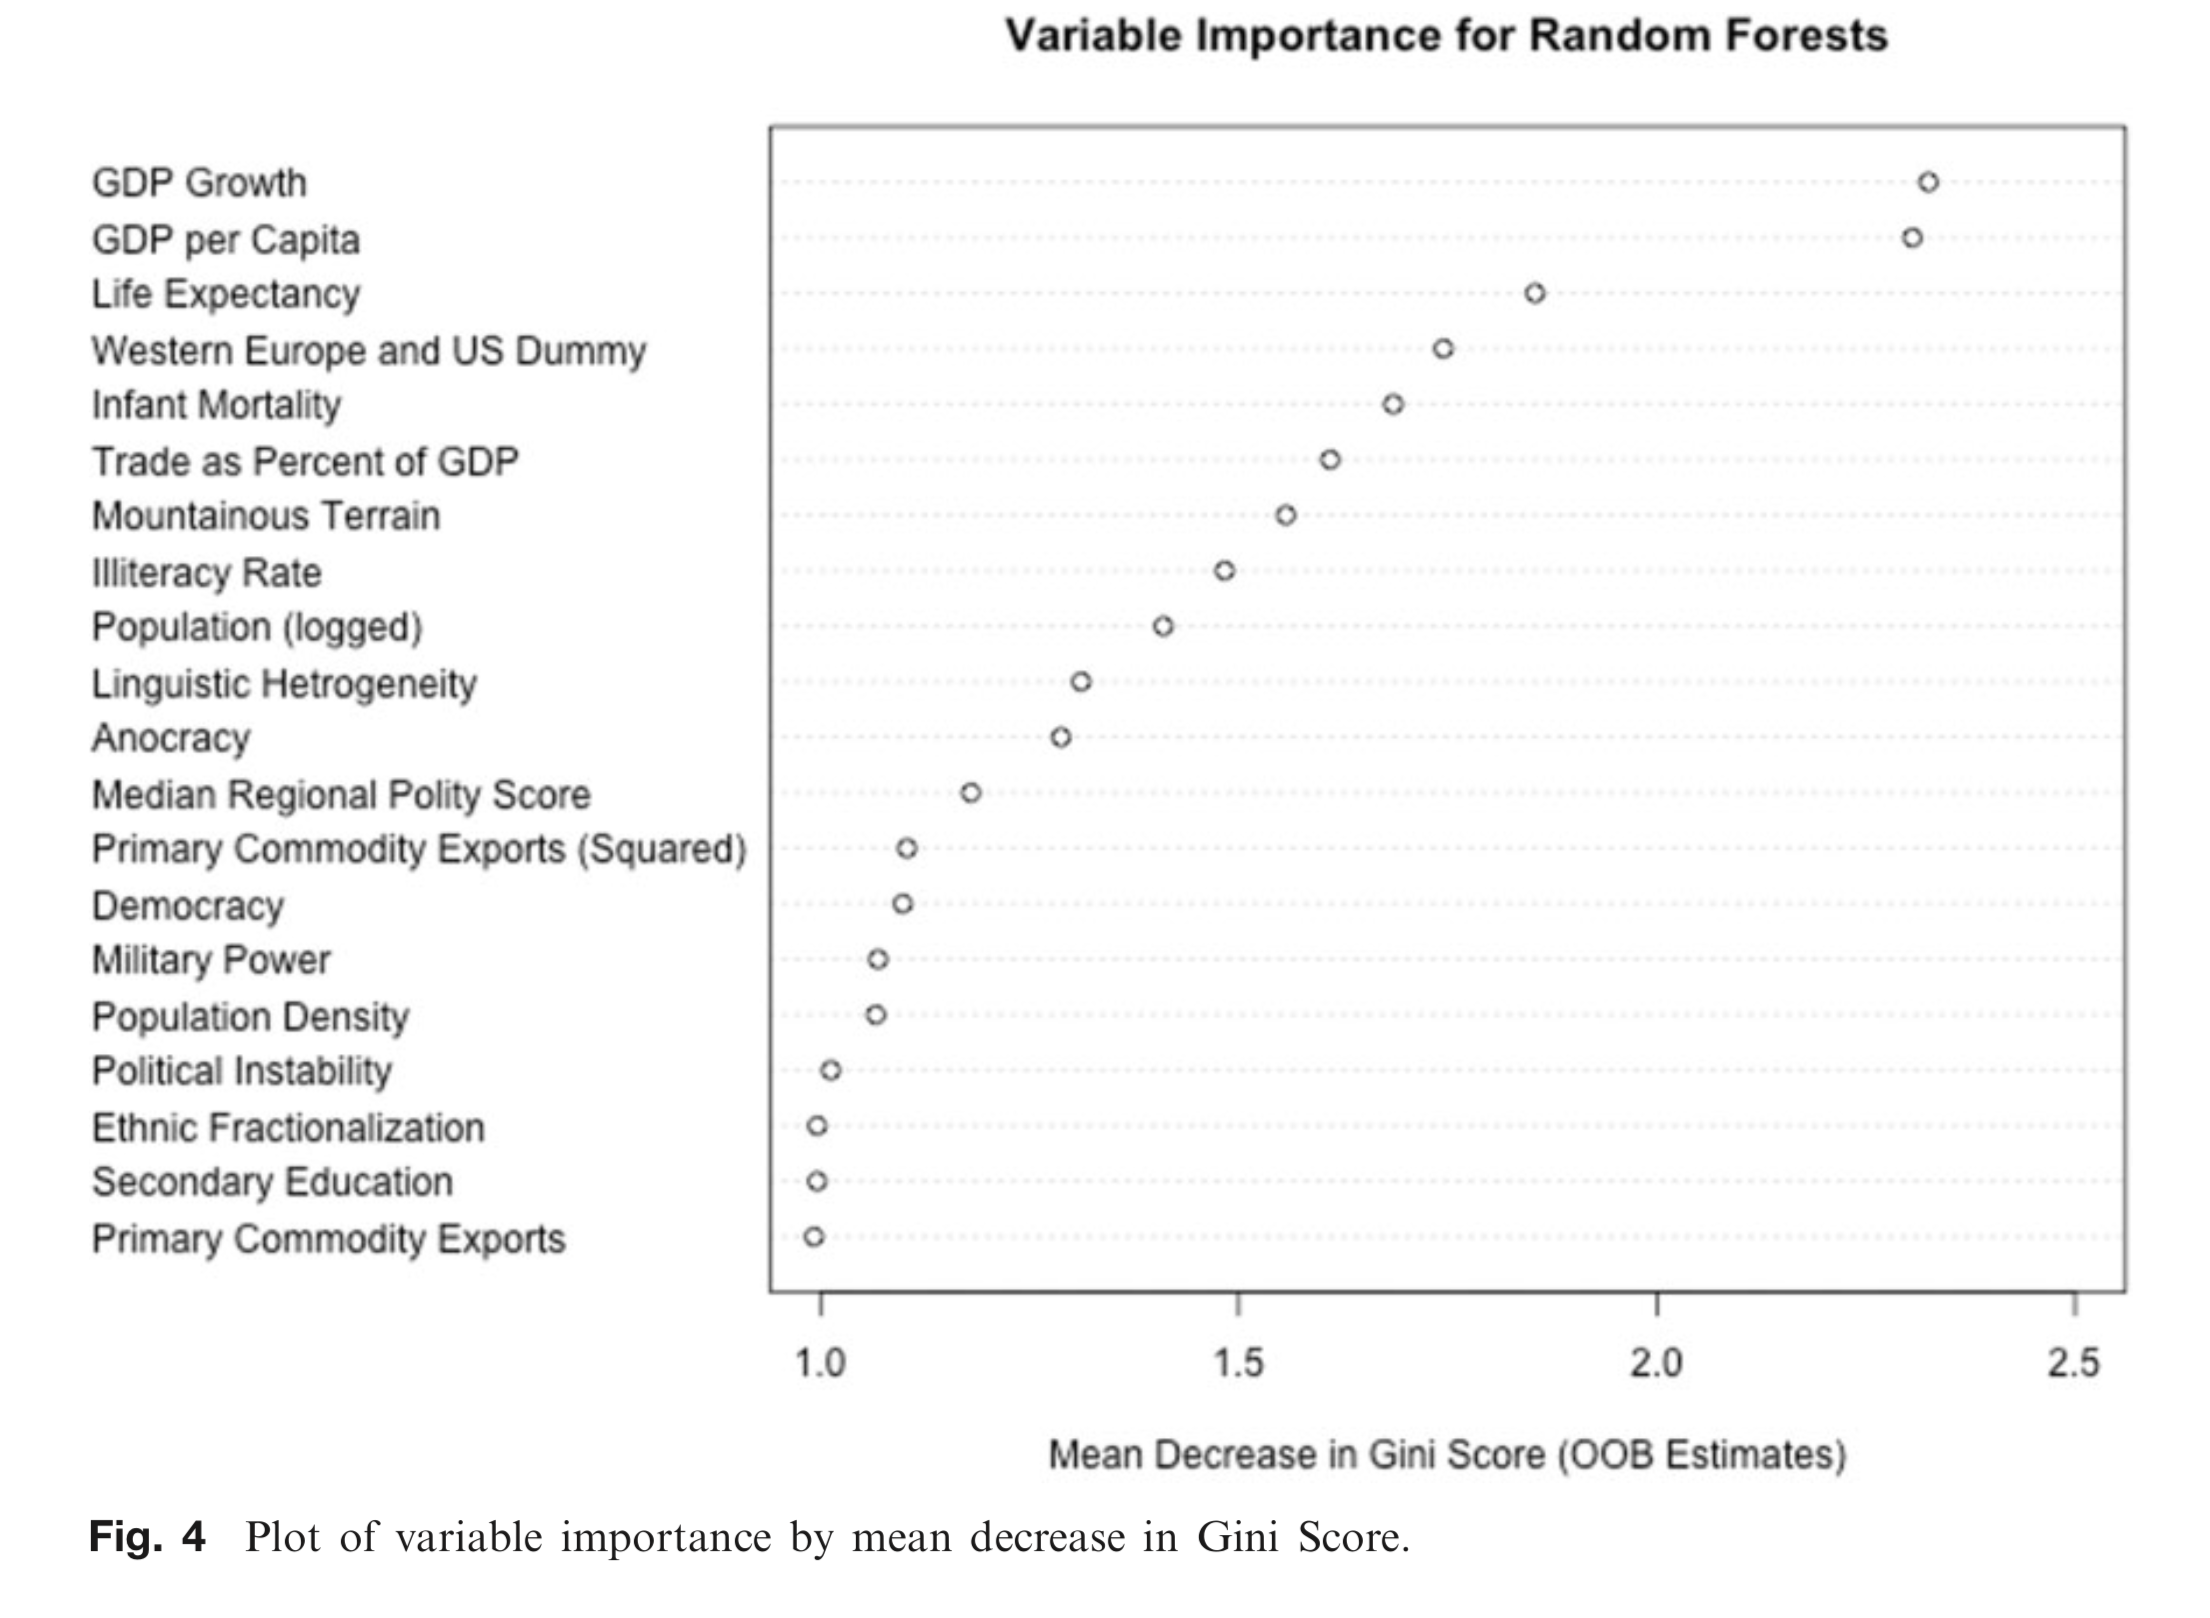
\includegraphics[width=0.45\textwidth]{figures/muchlinksi_comparing_2016_fig4}  \phantom{12345} 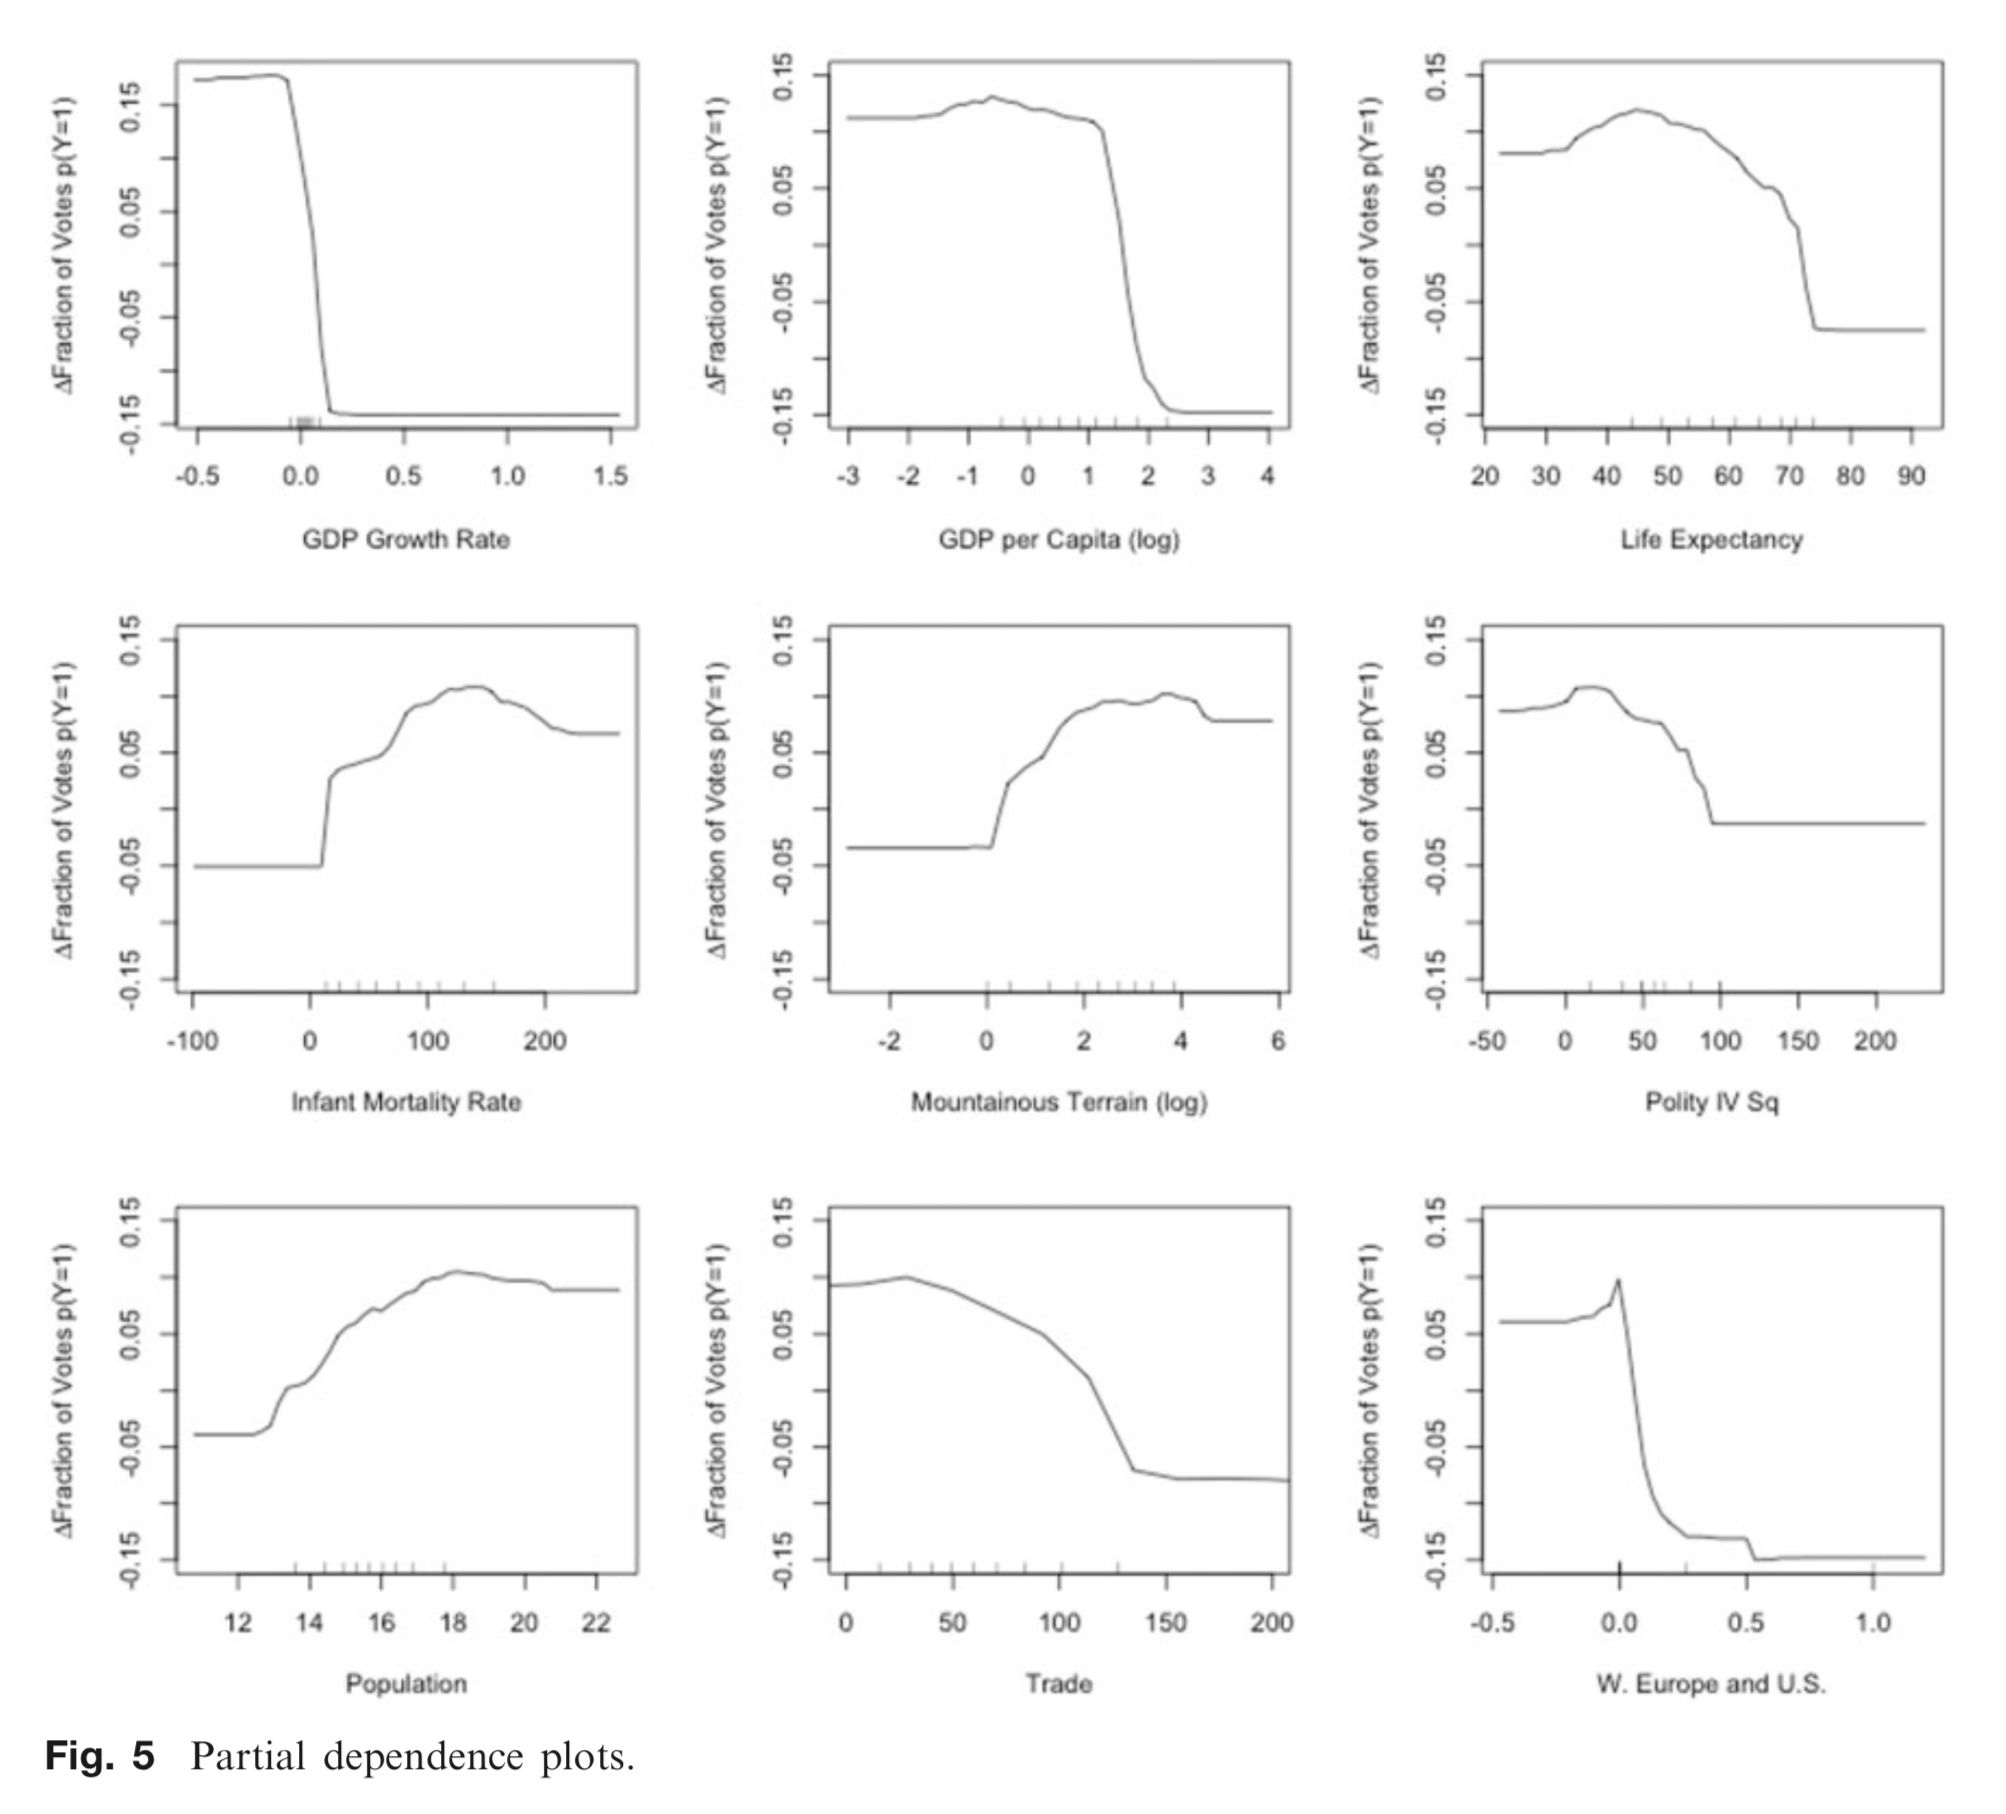
\includegraphics[width=0.45\textwidth]{figures/muchlinksi_comparing_2016_fig5} 
\end{center}

\pause
\begin{itemize}
\item I'm not sure I believe this. What are the units?
\pause
\item Recall Arvind's concerns about correlated predictors
\pause
\item If we did this with a slightly different implementation of random forest would we get the same results? What about another ML method?
\end{itemize}

\end{frame}
%%%%%%%%%%%%%%%%%%%%%%%%%%%
\begin{frame}
\frametitle{}

Assignment 2

\end{frame}
%%%%%%%%%%%%%%%%%%%%%%%%%%%
\begin{frame}
\frametitle{}

\begin{itemize}
\item It is very hard to tell what is happening in the comments and replies without digging in, hence your assignment. But imagine what we happen if the code was not available!
\pause
\item Can we use predictive models to learn about the data generating process?
\pause
\item What is a good way to measure generalization performance when there is measurement uncertainty?
\end{itemize}

\end{frame}
%%%%%%%%%%%%%%%%%%%%%%%%%%%
\begin{frame}
\frametitle{}

\begin{center}
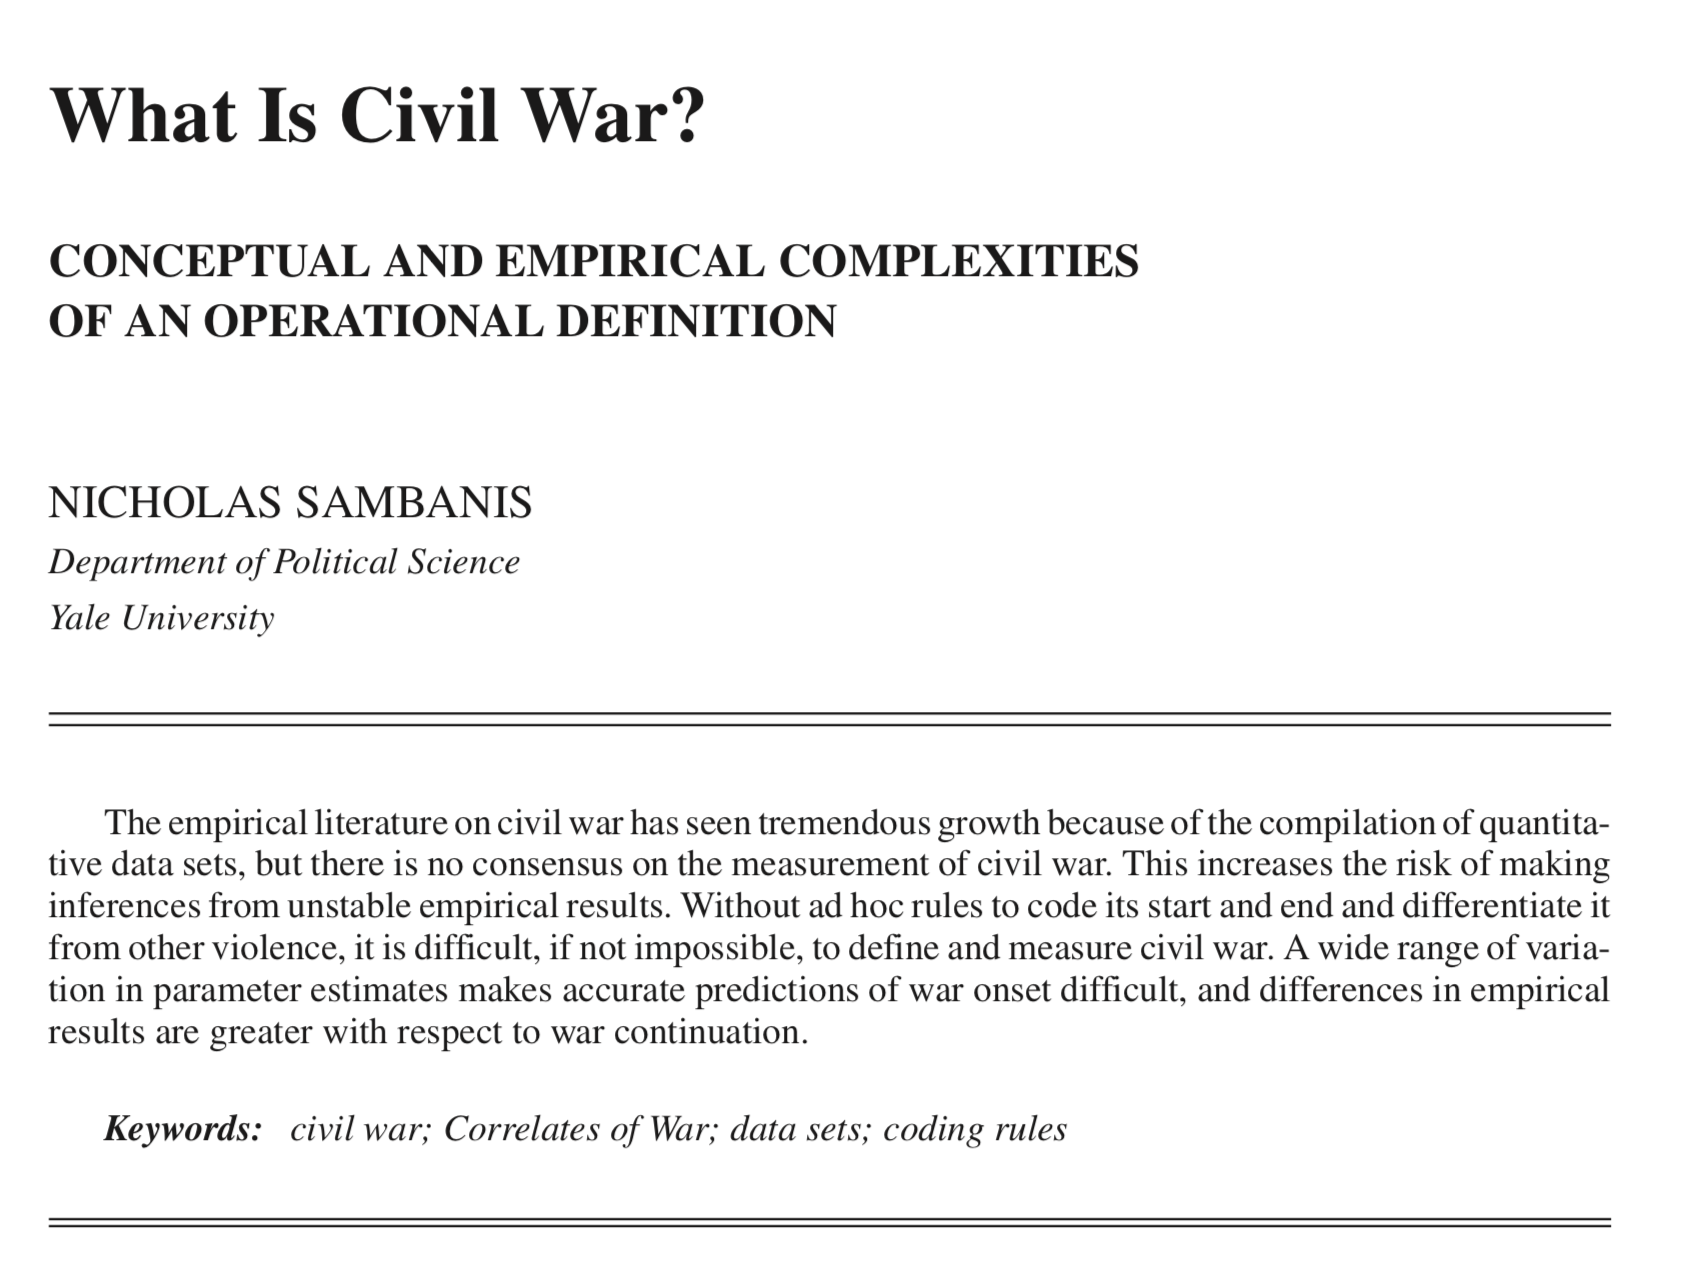
\includegraphics[width=0.9\textwidth]{figures/sambanis_what_2004_title}
\end{center}

\end{frame}
%%%%%%%%%%%%%%%%%%%%%%%%%%%
\begin{frame}
\frametitle{}

\begin{center}
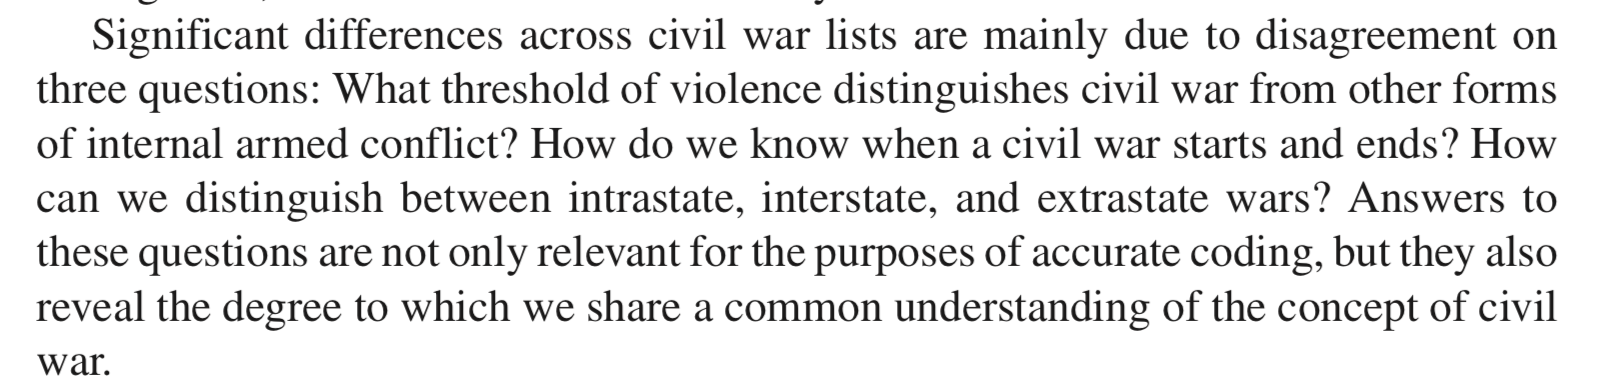
\includegraphics[width=0.9\textwidth]{figures/sambanis_what_2004_para}
\end{center}

12 different measures of civil wars. Does this matter? Should we standardize on one definition? Think back to ImageNet.

\end{frame}
%%%%%%%%%%%%%%%%%%%%%%%%%%%
\begin{frame}
\frametitle{}

\begin{center}
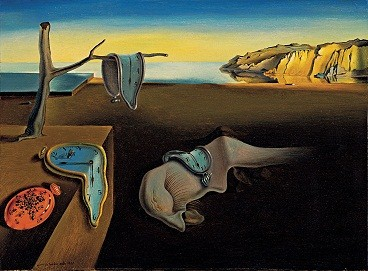
\includegraphics[width=0.8\textwidth]{figures/The_Persistence_of_Memory}
\end{center}

\vfill
\tiny{\url{https://upload.wikimedia.org/wikipedia/en/d/dd/The_Persistence_of_Memory.jpg}}

\end{frame}
%%%%%%%%%%%%%%%%%%%%%%%%%%%
\begin{frame}
\frametitle{}

\begin{itemize}
\item What is a good way to measure generalization performance when the data has structure (focus on time)? 
\pause
\item Should we use the future to predict the past? Should we use the present to predict the present?
\end{itemize}

\end{frame}
%%%%%%%%%%%%%%%%%%%%%%%%%%%
\begin{frame}
\frametitle{}

\begin{center}
\only<1>{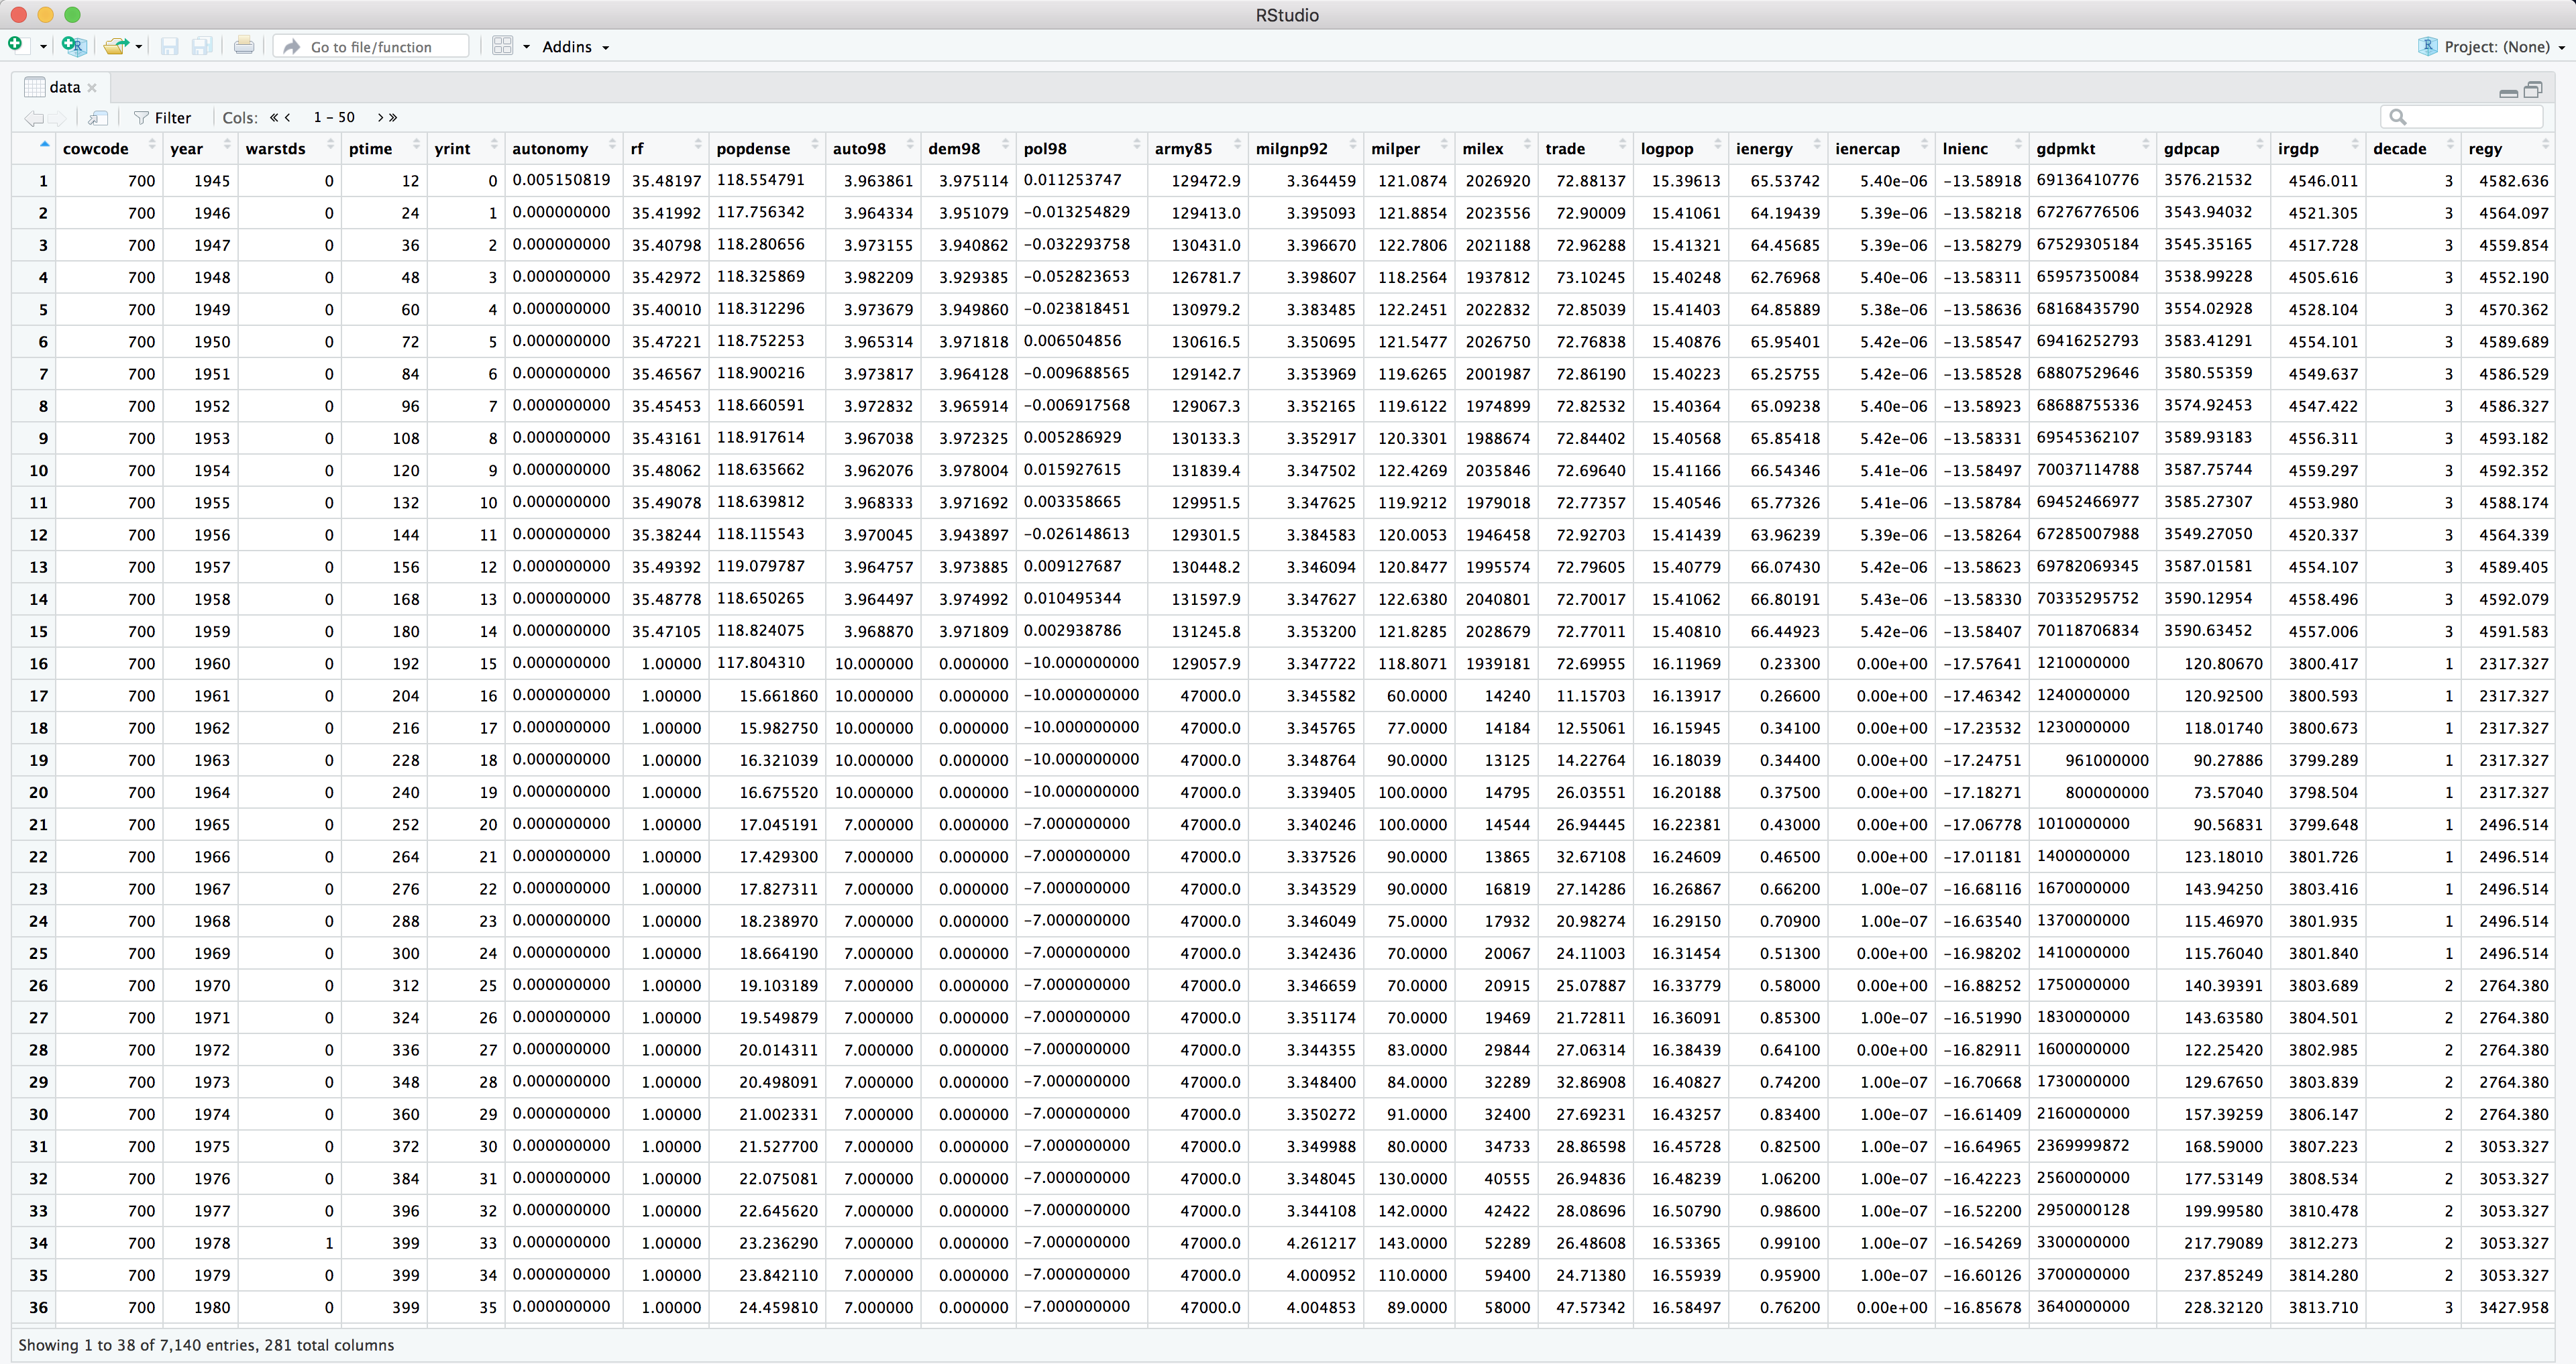
\includegraphics[width=0.9\textwidth]{figures/muchlinksi_data}}%
\only<2>{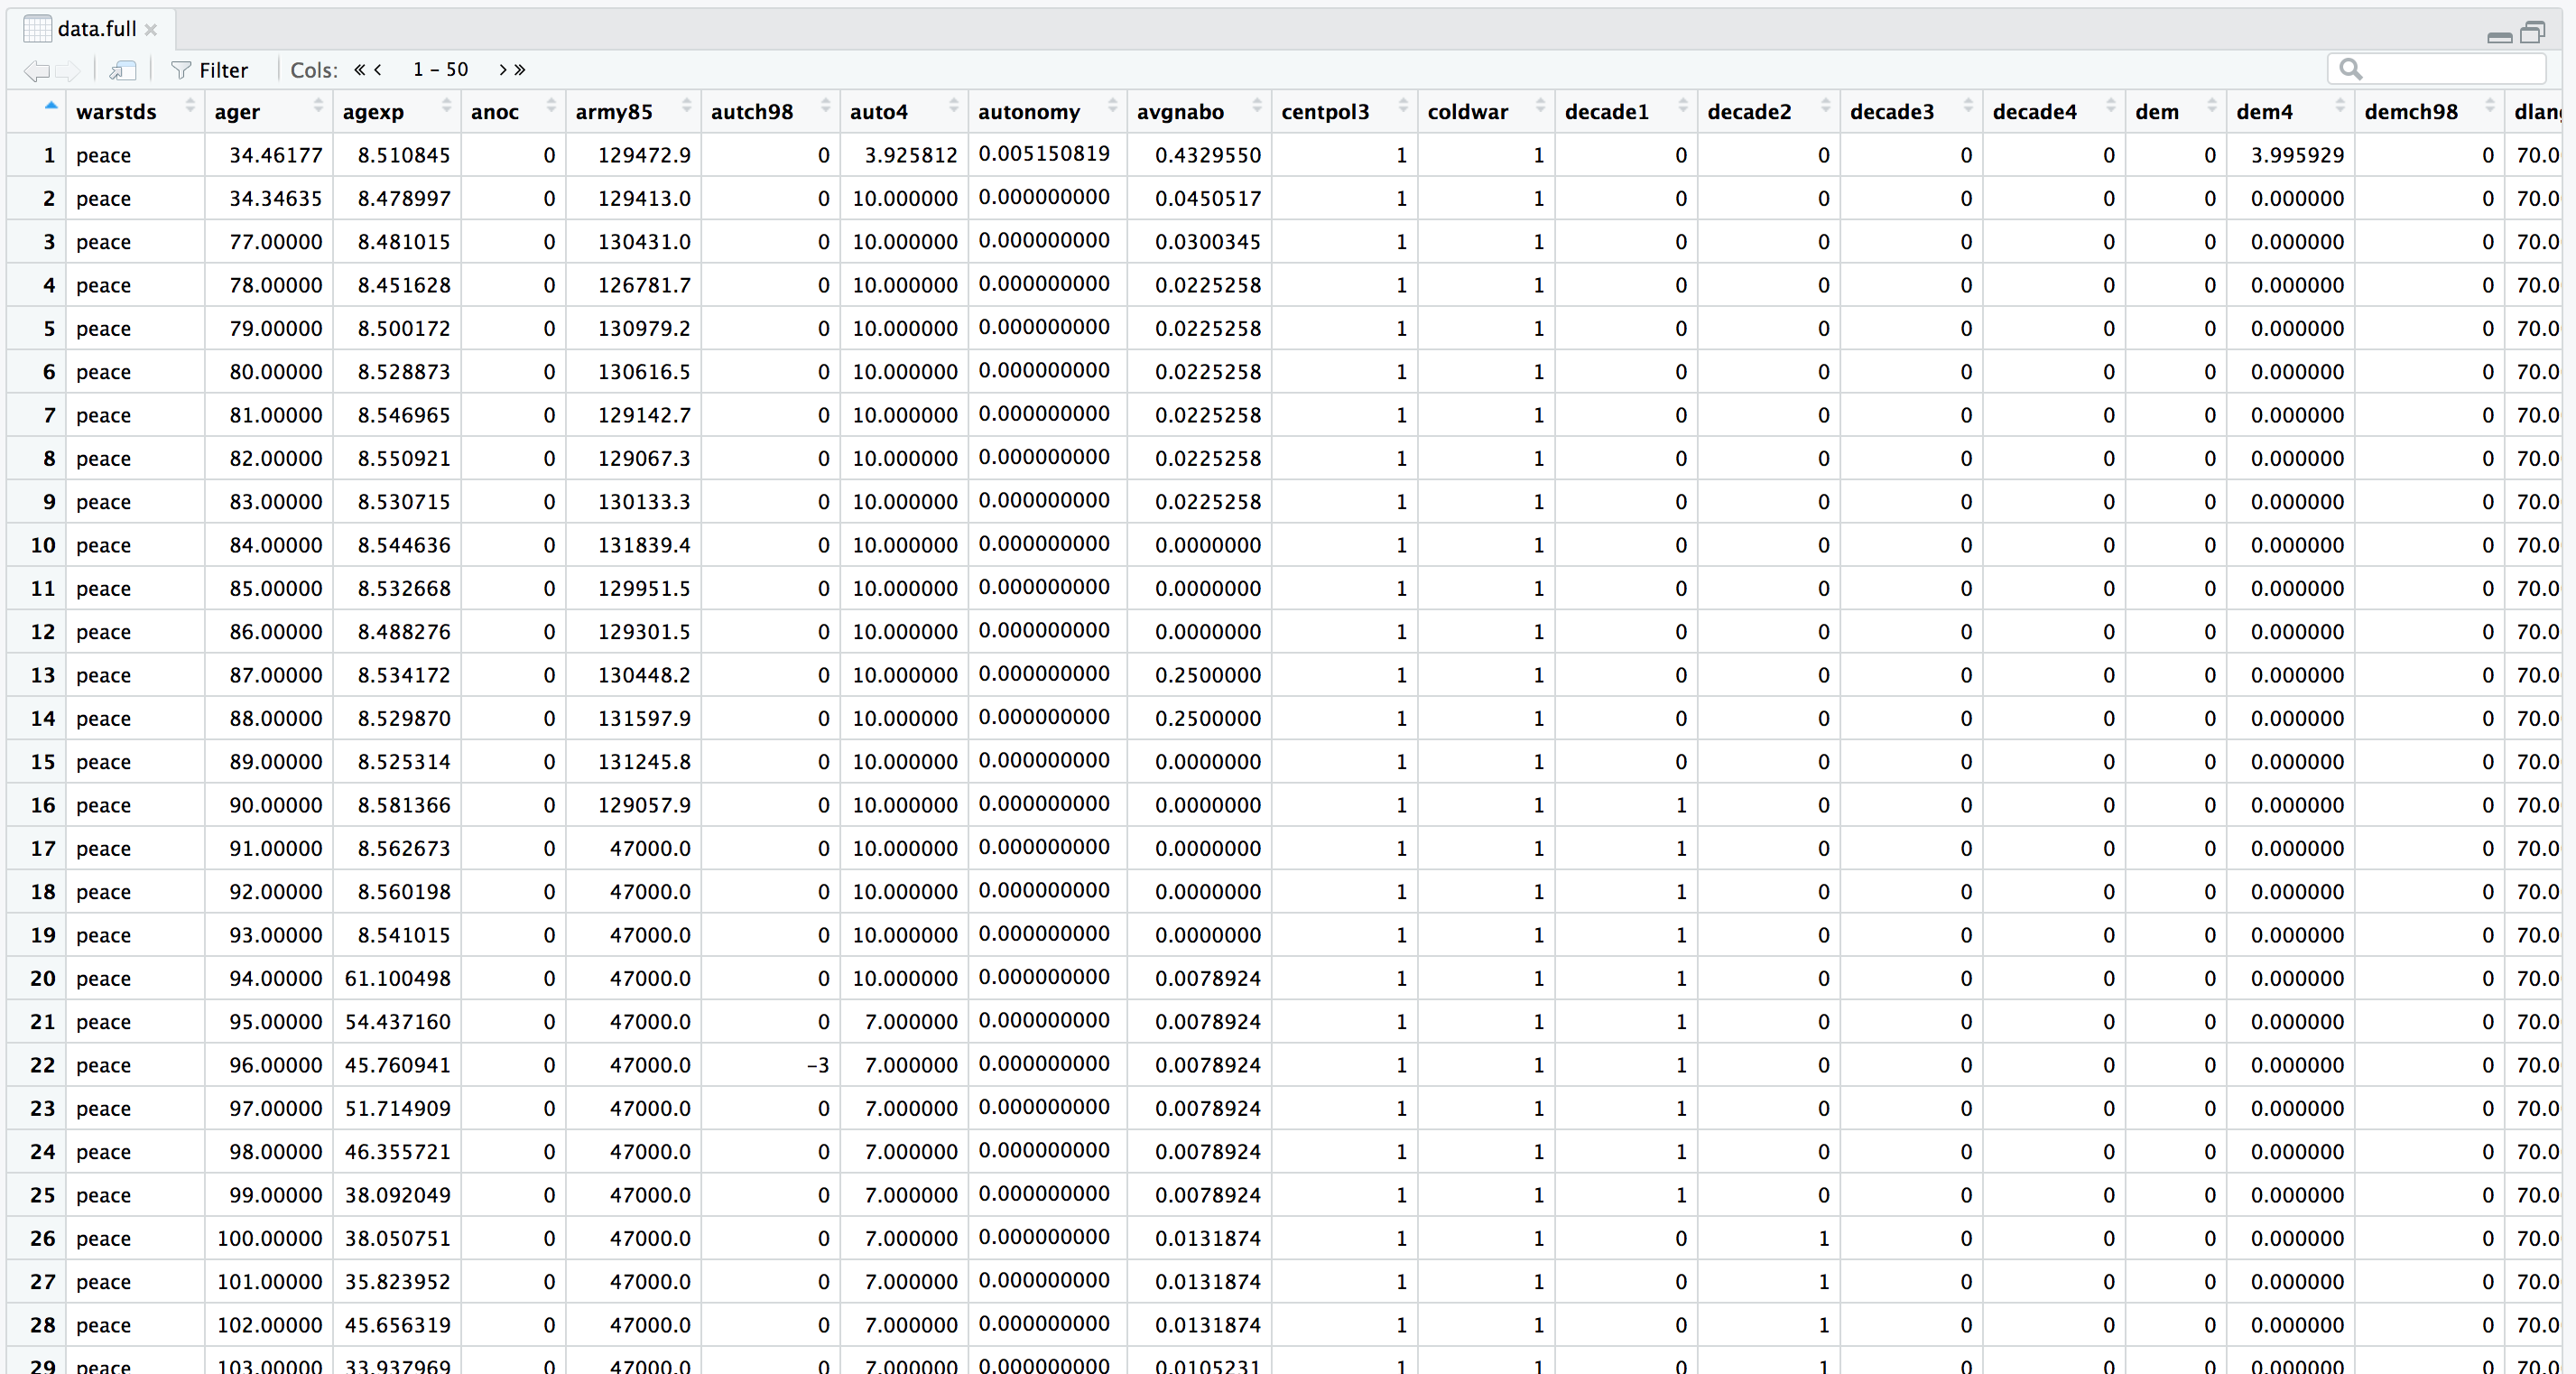
\includegraphics[width=0.9\textwidth]{figures/muchlinksi_data_used}}%
\end{center}

\pause
\vfill
Drops year and country code. These are never used in the paper (as far as I can tell).

\end{frame}
%%%%%%%%%%%%%%%%%%%%%%%%%%
\begin{frame}
\frametitle{}

\begin{center}
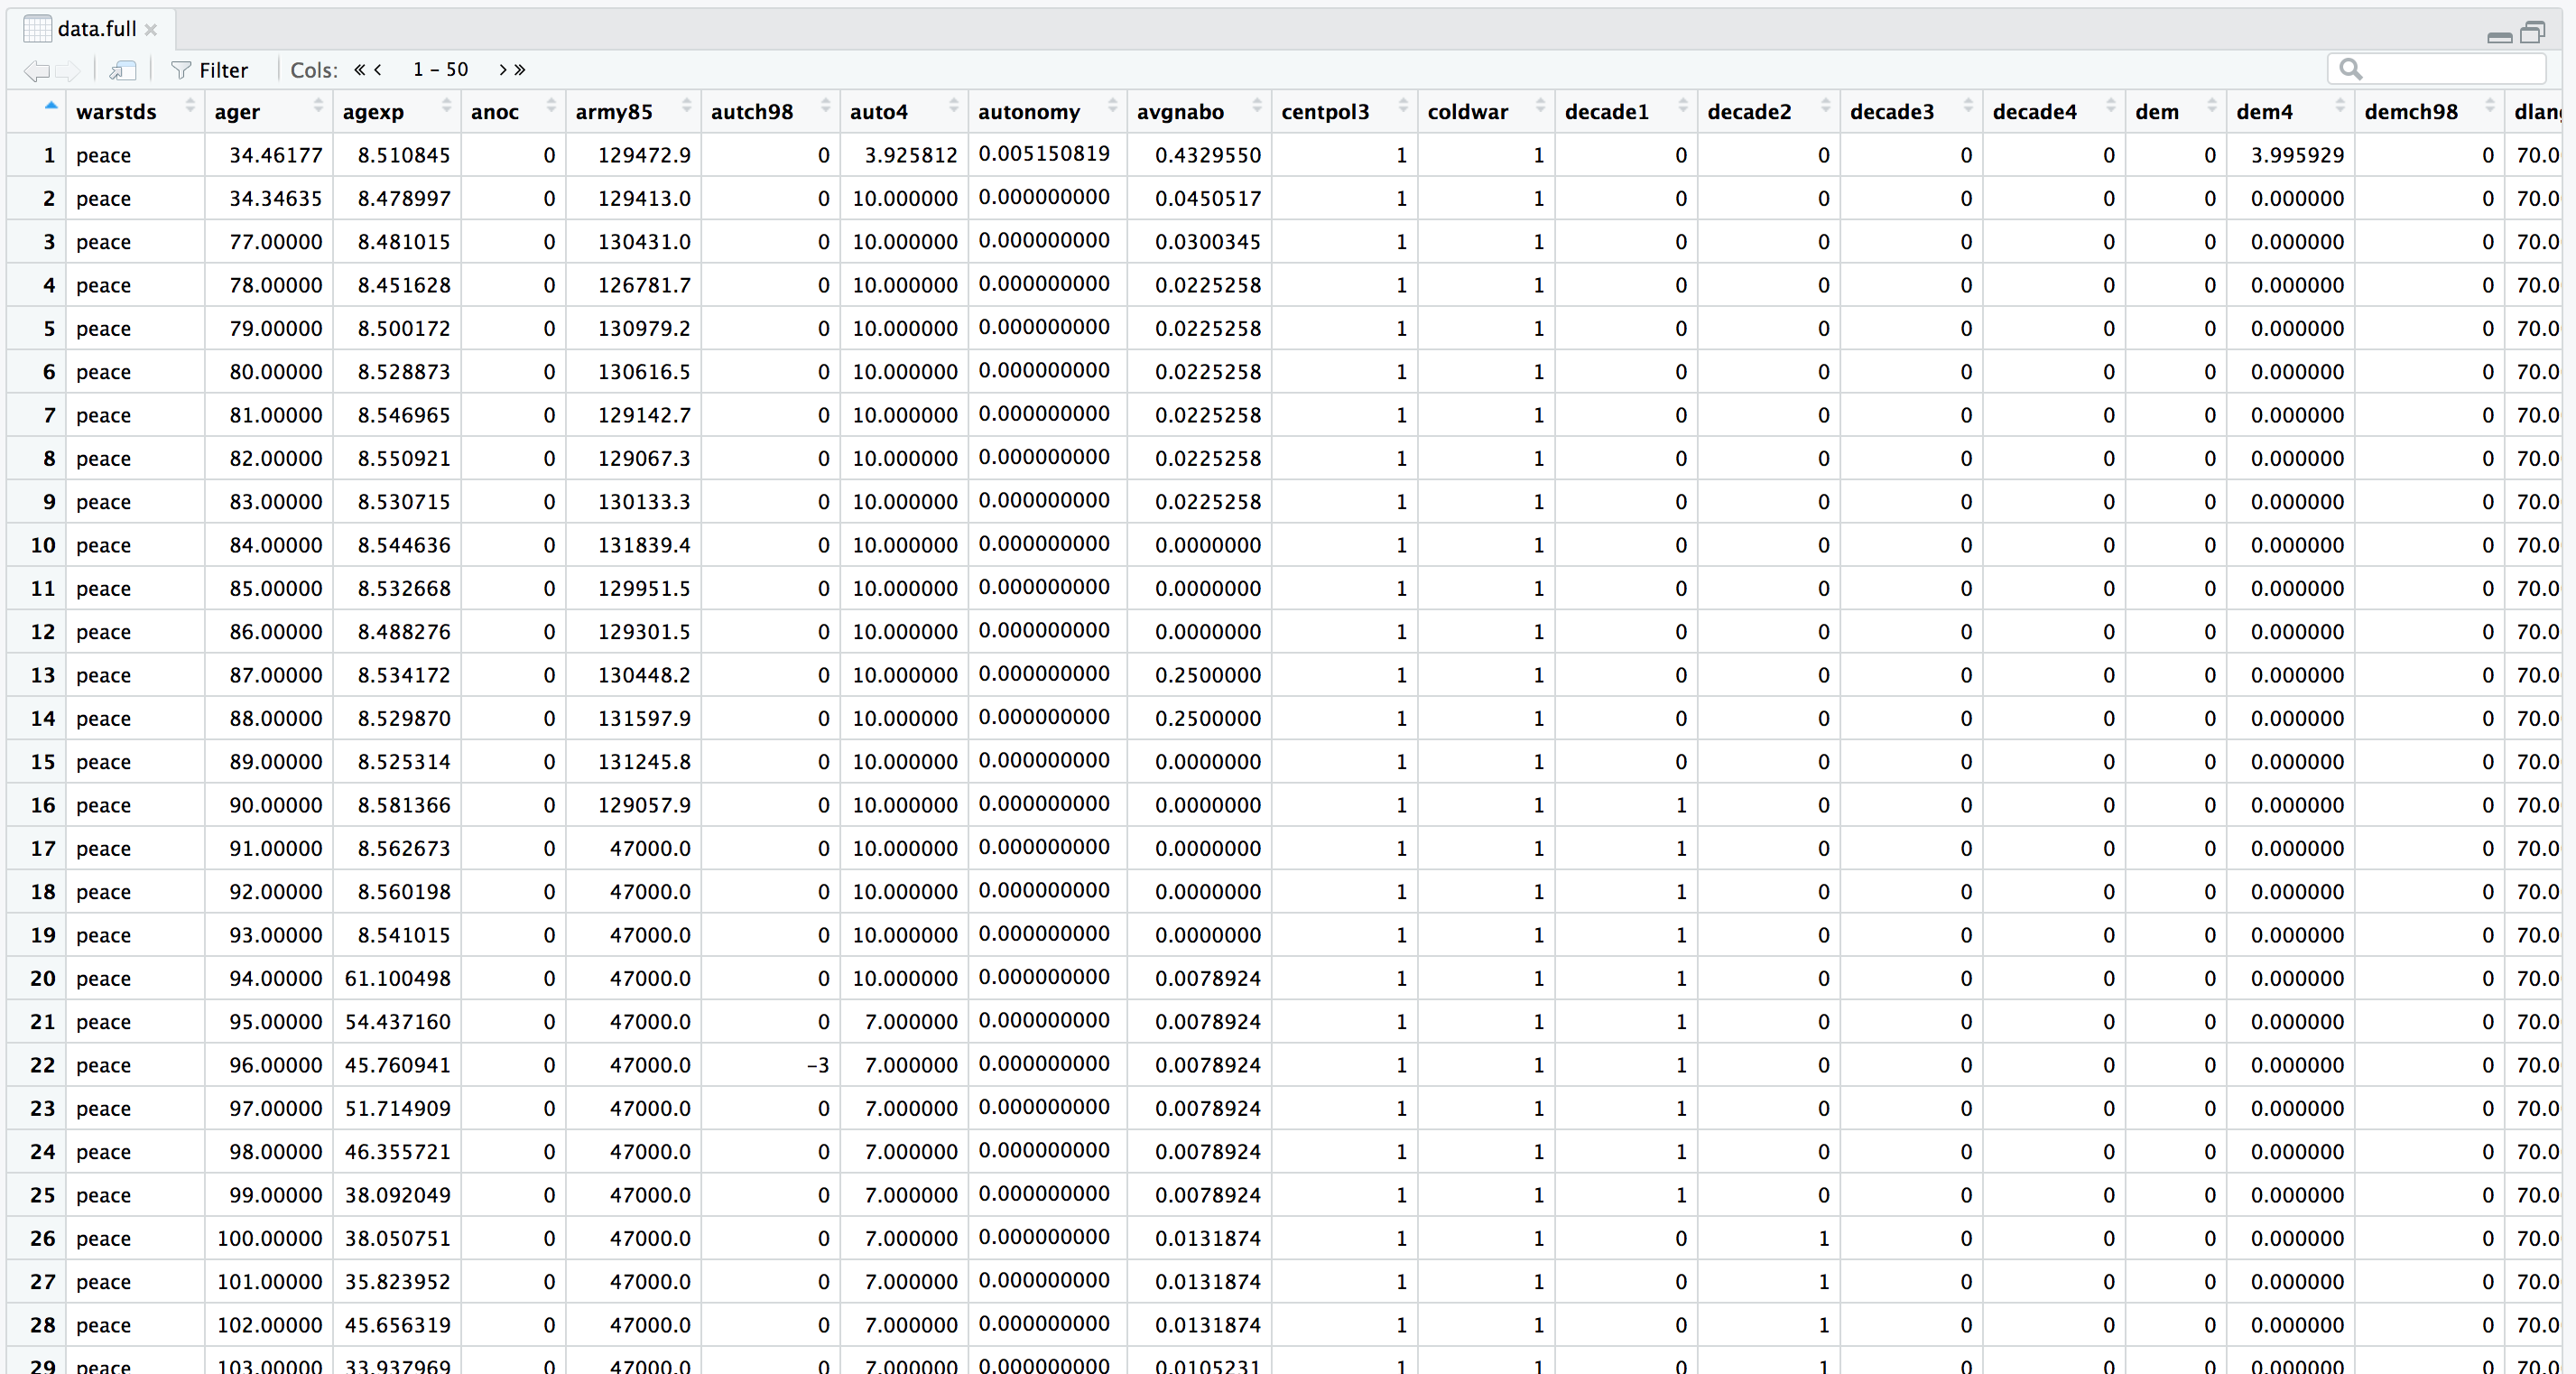
\includegraphics[width=0.6\textwidth]{figures/muchlinksi_data_used}
\end{center}

\pause

\phantom{12345}

\begin{center}
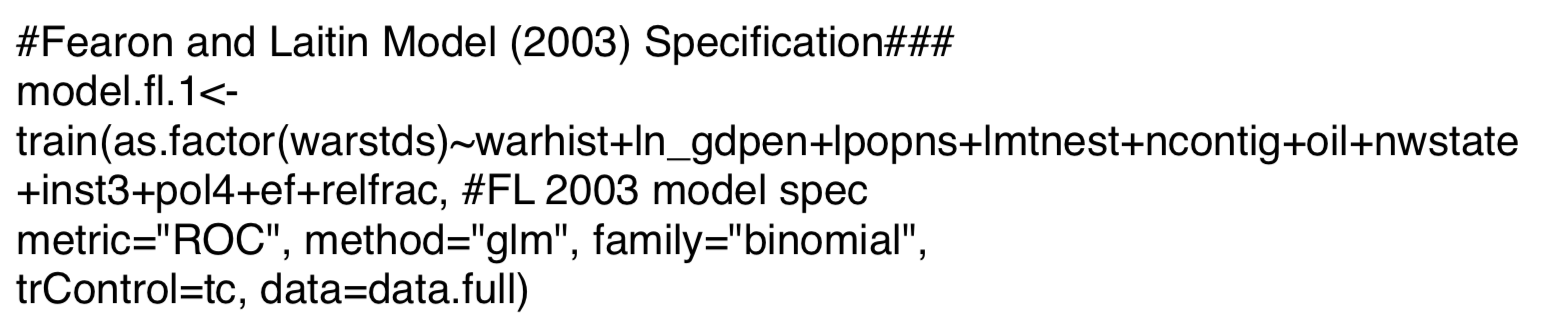
\includegraphics[width=0.9\textwidth]{figures/muchlinksi_fl}
\end{center}

\vfill
Uses the present to predict the present

\end{frame}
%%%%%%%%%%%%%%%%%%%%%%%%%%
\begin{frame}
\frametitle{}

Assignment 2

\end{frame}
%%%%%%%%%%%%%%%%%%%%%%%%%%%
\frame{\titlepage}


\end{document}
